\documentclass[11pt,a4paper]{report}

\usepackage{amsmath,amssymb}
\usepackage{physics}
\usepackage{geometry}
\usepackage{hyperref}
\usepackage{bm}
\usepackage{tikz}
\usetikzlibrary{arrows.meta,calc,positioning}


\geometry{margin=2.5cm}

\title{Gargantua\\
\large Physical and Mathematical Foundations of Photon Ray Tracing}
\author{}
\date{}

\begin{document}
\maketitle

\tableofcontents
\newpage

% ============================================================
\chapter{Schwarzschild Spacetime}

% ============================================================
\section{Introduction}

This document provides a complete physical and mathematical derivation
of the equations implemented in the \texttt{Gargantua} ray tracer.
The goal is not only to present final formulas, but to show
\emph{why each equation is introduced and how it follows from General Relativity}.

The document is written as a self-contained set of notes,
intended to bridge the gap between theoretical GR and practical numerical implementation.

We focus on:
\begin{itemize}
  \item null geodesics in Schwarzschild spacetime,
  \item reduction of spacetime geodesics to an orbit equation,
  \item geometric construction of initial conditions from ray data,
  \item numerical integration using Runge--Kutta methods.
\end{itemize}

Geometric units $G=c=1$ are used throughout.

% ============================================================
\section{Spacetime Interval and Metric}

In General Relativity, gravity is not a force but a manifestation of spacetime geometry.
This geometry is encoded in the metric tensor $g_{\mu\nu}$.

The invariant spacetime interval between two infinitesimally close events is

\begin{equation}
ds^2 = g_{\mu\nu}\,dx^\mu\,dx^\nu.
\end{equation}

This quantity plays the role analogous to distance in Euclidean space.
All physical predictions must be invariant under coordinate transformations,
which is why the metric formulation is fundamental.

A particle trajectory is a curve $x^\mu(\lambda)$ parametrized
by an affine parameter $\lambda$.

% ============================================================
\section{Why Extremize the Action}

Free particles move along paths that extremize the spacetime interval.
This principle generalizes the principle of least action from classical mechanics.

The action is defined as

\begin{equation}
S = \int ds.
\end{equation}

The actual physical trajectory is the one for which $\delta S = 0$.

For computational purposes, it is inconvenient to work with the square root in $ds$.
Fortunately, extremizing $S=\int ds$ is equivalent to extremizing

\begin{equation}
S = \int \mathcal{L}\,d\lambda,
\qquad
\mathcal{L} = \frac{1}{2} g_{\mu\nu}
\frac{dx^\mu}{d\lambda}
\frac{dx^\nu}{d\lambda}.
\end{equation}

This quadratic Lagrangian produces the same geodesic equations
and greatly simplifies the mathematics.

The parameter $\lambda$ is called an \emph{affine parameter}.
For photons, it does not correspond to proper time,
but still parametrizes the curve consistently.

% ============================================================
\section{Schwarzschild Spacetime}

The Schwarzschild metric describes spacetime outside a static,
spherically symmetric mass $M$.

In Schwarzschild coordinates $(t,r,\theta,\phi)$:

\begin{equation}
ds^2 =
-\left(1-\frac{2M}{r}\right)dt^2
+\left(1-\frac{2M}{r}\right)^{-1}dr^2
+r^2 d\theta^2
+r^2\sin^2\theta\,d\phi^2.
\end{equation}

Due to spherical symmetry, any geodesic can be rotated
into the equatorial plane:

\begin{equation}
\theta = \frac{\pi}{2}.
\end{equation}

The metric then reduces to

\begin{equation}
ds^2 =
-\left(1-\frac{2M}{r}\right)dt^2
+\left(1-\frac{2M}{r}\right)^{-1}dr^2
+r^2 d\phi^2.
\end{equation}

The event horizon is located at

\begin{equation}
r_s = 2M.
\end{equation}

% ============================================================
\section{Geodesic Lagrangian}

Substituting the Schwarzschild metric into the quadratic action yields

\begin{equation}
\mathcal{L}
=
\frac{1}{2}\left[
-\left(1-\frac{2M}{r}\right)\dot{t}^2
+\left(1-\frac{2M}{r}\right)^{-1}\dot{r}^2
+r^2\dot{\phi}^2
\right],
\end{equation}

where dots denote derivatives with respect to the affine parameter $\lambda$.

For photons (null geodesics), the constraint

\begin{equation}
ds^2 = 0
\end{equation}

must hold along the trajectory.

% ============================================================
\section{Conserved Quantities from Symmetries}

Because the Lagrangian does not depend explicitly on $t$ or $\phi$,
their conjugate momenta are conserved.
This is a direct consequence of Noether's theorem.

\subsection{Energy}

\begin{equation}
p_t = \frac{\partial\mathcal{L}}{\partial\dot{t}}
= -\left(1-\frac{2M}{r}\right)\dot{t}.
\end{equation}

We define the conserved energy

\begin{equation}
E = \left(1-\frac{2M}{r}\right)\dot{t}.
\end{equation}

\subsection{Angular Momentum}

\begin{equation}
p_\phi = \frac{\partial\mathcal{L}}{\partial\dot{\phi}}
= r^2\dot{\phi}.
\end{equation}

We define the conserved angular momentum

\begin{equation}
L = r^2\dot{\phi}.
\end{equation}

% ============================================================
\section{Radial Equation of Motion}

For null geodesics, impose the constraint

\begin{equation}
g_{\mu\nu}\dot{x}^\mu\dot{x}^\nu = 0.
\end{equation}

Substituting the metric and conserved quantities yields

\begin{equation}
\dot{r}^2
=
E^2
-
\left(1-\frac{2M}{r}\right)\frac{L^2}{r^2}.
\end{equation}

This equation describes radial motion in an effective potential.

% ============================================================
\section{Eliminating the Affine Parameter}

The shape of the trajectory does not depend on how it is parametrized.
We therefore eliminate $\lambda$ in favor of the angular coordinate $\phi$.

Using the chain rule:

\begin{equation}
\frac{dr}{d\phi}
=
\frac{dr/d\lambda}{d\phi/d\lambda}
=
\frac{\dot{r}}{\dot{\phi}}.
\end{equation}

Since $L=r^2\dot{\phi}$:

\begin{equation}
\dot{\phi} = \frac{L}{r^2}.
\end{equation}

Substituting yields

\begin{equation}
\left(\frac{dr}{d\phi}\right)^2
=
\frac{r^4}{L^2}
\left[
E^2
-
\left(1-\frac{2M}{r}\right)\frac{L^2}{r^2}
\right].
\end{equation}

% ============================================================
\section{Substitution $u = 1/r$}

Define the inverse radius

\begin{equation}
u = \frac{1}{r}.
\end{equation}

This substitution simplifies the equation and turns the orbit problem
into a differential equation for $u(\phi)$.

Using

\begin{equation}
\frac{dr}{d\phi} = -\frac{1}{u^2}\frac{du}{d\phi},
\end{equation}

we obtain

\begin{equation}
\left(\frac{du}{d\phi}\right)^2
=
\frac{1}{b^2}
-
u^2
+
2Mu^3,
\qquad
b=\frac{L}{E}.
\end{equation}

Differentiating with respect to $\phi$ gives the second-order orbit equation:

\begin{equation}
\boxed{
\frac{d^2u}{d\phi^2} + u = 3Mu^2.
}
\end{equation}

This equation fully determines photon trajectories.

% ============================================================
\section{Geometric Initial Conditions}

The numerical solver requires initial values

\[
u_0 = u(\phi_0),\qquad
v_0 = \left.\frac{du}{d\phi}\right|_{\phi_0}.
\]

Given initial position $\bm{p}_0$ and direction $\bm{d}$,
we construct a local polar basis around the black hole center $\bm{c}$:

\begin{align}
\hat{\bm{r}} &= \frac{\bm{p}_0-\bm{c}}{|\bm{p}_0-\bm{c}|},\\
\hat{\bm{\phi}} &= (-\hat{r}_y,\hat{r}_x).
\end{align}

Velocity decomposition:

\begin{equation}
\dot{\bm{r}} = \dot{r}\hat{\bm{r}} + r\dot{\phi}\hat{\bm{\phi}}.
\end{equation}

Thus:

\begin{align}
\dot{r} &= \bm{d}\cdot\hat{\bm{r}},\\
r\dot{\phi} &= \bm{d}\cdot\hat{\bm{\phi}}.
\end{align}

Using $u=1/r$, the initial slope is

\begin{equation}
\boxed{
v_0
=
-\frac{1}{r_0}
\frac{\bm{d}\cdot\hat{\bm{r}}}{\bm{d}\cdot\hat{\bm{\phi}}}.
}
\end{equation}

% ============================================================
\section{Numerical Integration: Runge--Kutta 4}

The orbit equation is written as a first-order system:

\begin{align}
\frac{du}{d\phi} &= v,\\
\frac{dv}{d\phi} &= -u + 3Mu^2.
\end{align}

This system is integrated using the classical fourth-order Runge--Kutta method.
RK4 evaluates the slope at multiple points inside each step,
providing high accuracy and stability for smooth trajectories.

% ============================================================
\section{Conclusion}

The Gargantua ray tracer implements photon trajectories
as null geodesics of Schwarzschild spacetime.
Each component of the code corresponds directly
to a well-defined physical and mathematical concept,
making the implementation both accurate and interpretable.


% ============================================================
% ============================================================
% ============================================================

\chapter{3D Ray Marching}

\section{Camera Model and Ray Generation}

\subsection{Overview}

In Gargantua, image formation is based on a \textbf{pinhole camera model}.
An image is produced by casting one ray per pixel from a single camera position
into the scene and evaluating physical interactions along that ray.

All rays:
\begin{itemize}
\item originate from the same camera position,
\item diverge into space according to the camera field of view,
\item form a rectangular pyramidal frustum.
\end{itemize}

\begin{figure}[h]
\centering
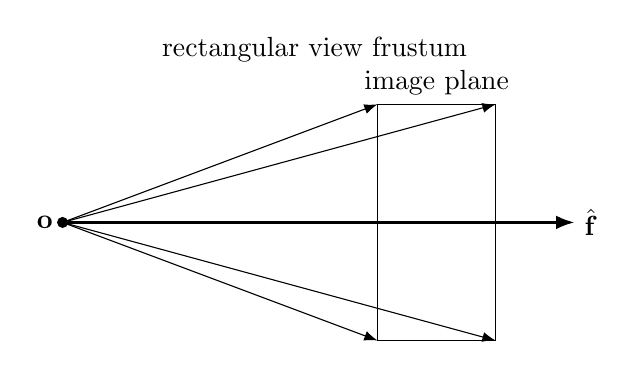
\begin{tikzpicture}[>=Latex, scale=1.0]

  % Camera position
  \coordinate (C) at (0,0);
  \fill (C) circle (2pt);
  \node[left] at (C) {$\mathbf{o}$};

  % Image plane (rectangle)
  \coordinate (TL) at (4, 1.5);
  \coordinate (TR) at (5.5, 1.5);
  \coordinate (BR) at (5.5,-1.5);
  \coordinate (BL) at (4,-1.5);

  \draw (TL) -- (TR) -- (BR) -- (BL) -- cycle;
  \node[above] at ($(TL)!0.5!(TR)$) {image plane};

  % Frustum edges (camera to plane corners)
  \draw[->] (C) -- (TL);
  \draw[->] (C) -- (TR);
  \draw[->] (C) -- (BR);
  \draw[->] (C) -- (BL);

  % Forward direction
  \draw[thick,->] (C) -- (6.5,0) node[right] {$\hat{\mathbf{f}}$};

  % Side edges (visual frustum volume hint)
  \draw[dashed] (TL) -- (BL);
  \draw[dashed] (TR) -- (BR);

  % Annotation
  \node at (3.2,2.2) {rectangular view frustum};

\end{tikzpicture}
\caption{Rectangular camera frustum. All rays originate at the camera position and pass through the corners of the image plane.}
\end{figure}



No projection of world points is performed.
Only ray directions are generated.

\subsection{Camera State}

A camera is defined by:
\begin{itemize}
\item $\mathbf{o} \in \mathbb{R}^3$ -- camera position,
\item $\mathbf{f} \in \mathbb{R}^3$ -- forward (view) direction,
\item $\mathbf{u}_{hint} \in \mathbb{R}^3$ -- preferred up direction,
\item $\mathrm{FOV}_x$, $\mathrm{FOV}_y$ -- horizontal and vertical field of view.
\end{itemize}

The forward vector defines the normal of the image plane.
The up vector is a \textbf{hint only} and does not need to be perpendicular to the forward direction.

\subsection{Camera Basis Construction}

From the provided vectors, an orthonormal camera basis is constructed:

\[
\hat{\mathbf{f}} = \frac{\mathbf{f}}{\|\mathbf{f}\|}
\]

\[
\hat{\mathbf{r}} = \frac{\hat{\mathbf{f}} \times \mathbf{u}_{hint}}{\|\hat{\mathbf{f}} \times \mathbf{u}_{hint}\|}
\]

\[
\hat{\mathbf{u}} = \hat{\mathbf{r}} \times \hat{\mathbf{f}}
\]

The resulting basis satisfies:

\[
\hat{\mathbf{f}} \cdot \hat{\mathbf{r}} =
\hat{\mathbf{f}} \cdot \hat{\mathbf{u}} =
\hat{\mathbf{r}} \cdot \hat{\mathbf{u}} = 0
\]

This construction resolves the roll ambiguity of the camera.

If $\hat{\mathbf{f}}$ is nearly parallel to $\mathbf{u}_{hint}$,
a fallback up vector is selected automatically.


\begin{figure}[h]
\centering
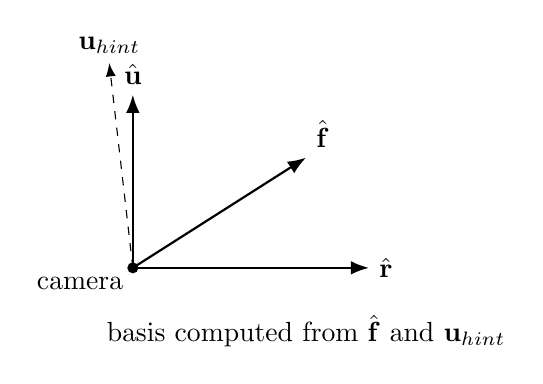
\begin{tikzpicture}[>=Latex, scale=1.0]
  \coordinate (O) at (0,0);
  \draw[thick,->] (O) -- (3,0) node[right] {$\hat{\mathbf{r}}$};
  \draw[thick,->] (O) -- (0,2.2) node[above] {$\hat{\mathbf{u}}$};
  \draw[thick,->] (O) -- (2.2,1.4) node[above right] {$\hat{\mathbf{f}}$};

  % Up hint (dashed)
  \draw[dashed,->] (O) -- (-0.3,2.6) node[above] {$\mathbf{u}_{hint}$};

  \fill (O) circle (2pt);
  \node[below left] at (O) {camera};

  \node at (2.2,-0.8) {basis computed from $\hat{\mathbf{f}}$ and $\mathbf{u}_{hint}$};
\end{tikzpicture}
\caption{The camera basis vectors (forward, right, up). The provided $\mathbf{u}_{hint}$ is a preference used to resolve roll.}
\end{figure}


\subsection{Image Plane Parameterization}

An imaginary image plane is defined in camera space at unit distance.
Its physical distance is irrelevant; only ray directions matter.

Plane extents are given by:

\[
x \in [-\tan(\mathrm{FOV}_x/2), \tan(\mathrm{FOV}_x/2)]
\]

\[
y \in [-\tan(\mathrm{FOV}_y/2), \tan(\mathrm{FOV}_y/2)]
\]

For an image of size $(H, W)$, each pixel $(i, j)$ is assigned coordinates:

\[
x_j = \mathrm{linspace}(-\tan(\mathrm{FOV}_x/2), \tan(\mathrm{FOV}_x/2))
\]

\[
y_i = \mathrm{linspace}(\tan(\mathrm{FOV}_y/2), -\tan(\mathrm{FOV}_y/2))
\]


\begin{figure}[h]
\centering
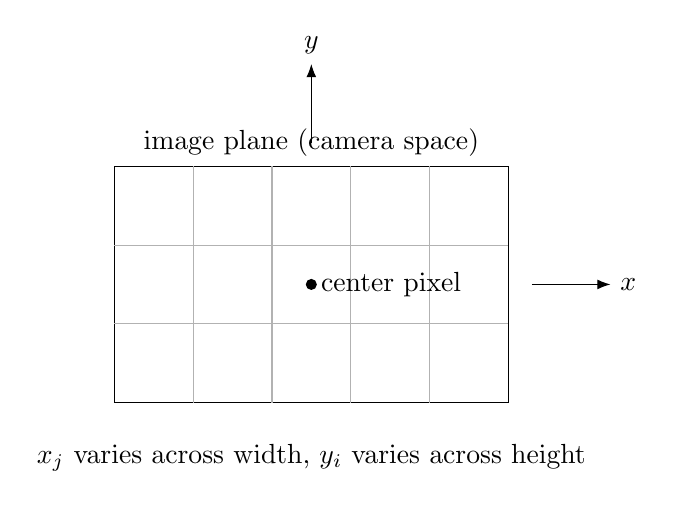
\begin{tikzpicture}[>=Latex, scale=1.0]
  % Image plane
  \draw (0,0) rectangle (5,3);
  \node[above] at (2.5,3) {image plane (camera space)};

  % Grid
  \foreach \x in {1,2,3,4} { \draw[gray!60] (\x,0) -- (\x,3); }
  \foreach \y in {1,2} { \draw[gray!60] (0,\y) -- (5,\y); }

  % Center pixel
  \fill (2.5,1.5) circle (2pt);
  \node[right] at (2.5,1.5) {center pixel};

  % Axes labels
  \draw[->] (5.3,1.5) -- (6.3,1.5) node[right] {$x$};
  \draw[->] (2.5,3.3) -- (2.5,4.3) node[above] {$y$};

  \node at (2.5,-0.7) {$x_j$ varies across width, $y_i$ varies across height};
\end{tikzpicture}
\caption{Each pixel corresponds to a point on the image plane parameterized by $(x_j, y_i)$ in camera space.}
\end{figure}


\subsection{Ray Direction Generation}

For each pixel $(i, j)$, a ray direction is computed as:

\[
\mathbf{d}_{ij} =
\hat{\mathbf{f}} +
x_j \hat{\mathbf{r}} +
y_i \hat{\mathbf{u}}
\]

The final ray direction is normalized:

\[
\hat{\mathbf{d}}_{ij} =
\frac{\mathbf{d}_{ij}}{\|\mathbf{d}_{ij}\|}
\]

All ray directions are stored in a tensor:

\[
\mathrm{rd0} \in \mathbb{R}^{H \times W \times 3}
\]

Each entry $\mathrm{rd0}_{ij}$ is a unit vector in world coordinates.

\begin{figure}[h]
\centering
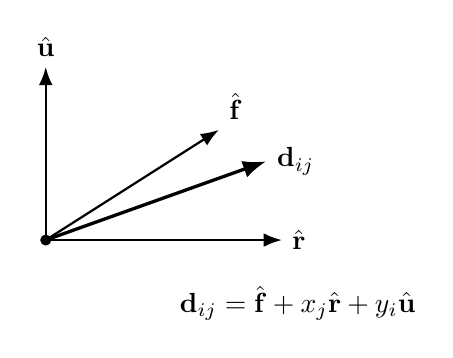
\begin{tikzpicture}[>=Latex, scale=1.0]
  \coordinate (O) at (0,0);

  % Basis
  \draw[thick,->] (O) -- (3,0) node[right] {$\hat{\mathbf{r}}$};
  \draw[thick,->] (O) -- (0,2.2) node[above] {$\hat{\mathbf{u}}$};
  \draw[thick,->] (O) -- (2.2,1.4) node[above right] {$\hat{\mathbf{f}}$};

  % Ray direction
  \draw[very thick,->] (O) -- (2.8,1.0) node[right] {$\mathbf{d}_{ij}$};

  % Labels
  \node at (3.2,-0.8) {$\mathbf{d}_{ij} = \hat{\mathbf{f}} + x_j\hat{\mathbf{r}} + y_i\hat{\mathbf{u}}$};

  \fill (O) circle (2pt);
\end{tikzpicture}
\caption{A pixel ray direction is formed by combining the camera basis vectors and then normalizing.}
\end{figure}



\subsection{Important Clarification}

The image plane is \textbf{not} a physical surface.
Rays do not stop or intersect it.
It exists only to parameterize ray directions.

All rays originate at the camera position $\mathbf{o}$.

\section{Ray Marching in 3D}

\subsection{Ray State Representation}

For image rendering, ray state is stored in batch form:

\begin{itemize}
\item $\mathbf{p} \in \mathbb{R}^{H \times W \times 3}$ -- current ray positions,
\item $\hat{\mathbf{d}} \in \mathbb{R}^{H \times W \times 3}$ -- ray directions,
\item $\mathrm{hit} \in \mathbb{R}^{H \times W}$ -- surface hit mask,
\item $\mathrm{fell\_in} \in \mathbb{R}^{H \times W}$ -- black hole capture mask.
\end{itemize}

Initially:

\[
\mathbf{p}_{ij} = \mathbf{o}
\quad \forall i, j
\]


\begin{figure}[h]
\centering
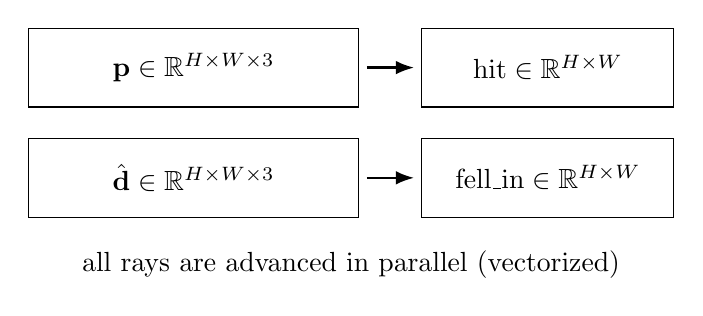
\begin{tikzpicture}[>=Latex, scale=1.0]
  % Boxes representing tensors
  \draw (0,0) rectangle (4.2,1.0);
  \node at (2.1,0.5) {$\mathbf{p} \in \mathbb{R}^{H\times W\times 3}$};

  \draw (0,-1.4) rectangle (4.2,-0.4);
  \node at (2.1,-0.9) {$\hat{\mathbf{d}} \in \mathbb{R}^{H\times W\times 3}$};

  \draw (5.0,0) rectangle (8.2,1.0);
  \node at (6.6,0.5) {$\mathrm{hit} \in \mathbb{R}^{H\times W}$};

  \draw (5.0,-1.4) rectangle (8.2,-0.4);
  \node at (6.6,-0.9) {$\mathrm{fell\_in} \in \mathbb{R}^{H\times W}$};

  % Arrow
  \draw[->, thick] (4.3,0.5) -- (4.9,0.5);
  \draw[->, thick] (4.3,-0.9) -- (4.9,-0.9);

  \node at (4.1,-2.0) {all rays are advanced in parallel (vectorized)};
\end{tikzpicture}
\caption{Ray marching stores the per-pixel ray state as batched arrays rather than nested loops.}
\end{figure}



\subsection{Signed Distance Field Evaluation}

For a sphere centered at $\mathbf{c}$ with radius $R$,
the signed distance field is:

\[
\mathrm{SDF}(\mathbf{p}) = \|\mathbf{p} - \mathbf{c}\| - R
\]

When evaluated in batch:

\[
\mathrm{SDF} : \mathbb{R}^{H \times W \times 3} \to \mathbb{R}^{H \times W}
\]

Each pixel ray receives an independent distance estimate.

\subsection{Marching Step}

At each iteration, rays are advanced by:

\[
\Delta s_{ij} =
\mathrm{clamp}(\mathrm{SDF}_{ij}, s_{min}, s_{max})
\]

\[
\mathbf{p}_{ij} \leftarrow
\mathbf{p}_{ij} + \hat{\mathbf{d}}_{ij} \Delta s_{ij}
\]

This ensures safe advancement without crossing surfaces.

\begin{figure}[h]
\centering
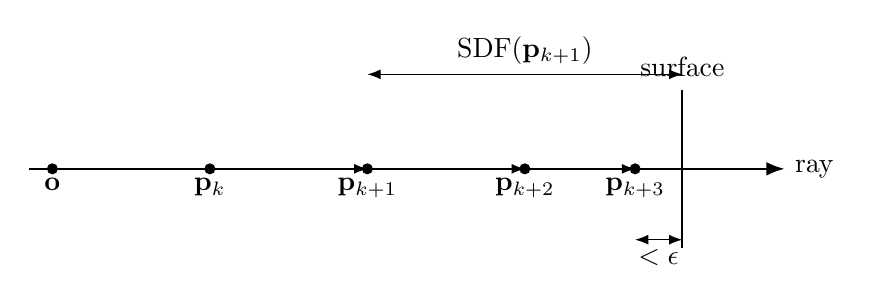
\begin{tikzpicture}[>=Latex, scale=1.0]

  % Ray axis
  \draw[thick,->] (-0.3,0) -- (9.3,0) node[right] {ray};

  % Camera
  \fill (0,0) circle (2pt);
  \node[below] at (0,0) {$\mathbf{o}$};

  % Surface
  \draw[thick] (8,-1.0) -- (8,1.0);
  \node[above] at (8,1.05) {surface};

  % Marching points
  \foreach \x/\lbl in {2/$\mathbf{p}_k$,4/$\mathbf{p}_{k+1}$,6/$\mathbf{p}_{k+2}$,7.4/$\mathbf{p}_{k+3}$} {
    \fill (\x,0) circle (2pt);
    \node[below] at (\x,0) {\lbl};
  }

  % Step arrows (kept simple)
  \draw[->] (2,0) -- (4,0);
  \draw[->] (4,0) -- (6,0);
  \draw[->] (6,0) -- (7.4,0);

  % One SDF illustration only (no repetition)
  \draw[<->] (4,1.2) -- (8,1.2);
  \node[above] at (6,1.2) {$\mathrm{SDF}(\mathbf{p}_{k+1})$};

  % Hit threshold
  \draw[<->] (7.4,-0.9) -- (8,-0.9);
  \node[below] at (7.7,-0.9) {$<\epsilon$};

\end{tikzpicture}
\caption{Ray marching advances a ray by safe steps estimated from the signed distance field. The ray hits the surface when the remaining distance drops below a small threshold $\epsilon$.}
\end{figure}



\subsection{Black Hole Bending}

Ray directions are updated according to a Newtonian bending model:

\[
\mathbf{r} = \mathbf{p} - \mathbf{c}_{BH}
\]

\[
\hat{\mathbf{d}} \leftarrow
\hat{\mathbf{d}} - M \frac{\mathbf{r}}{\|\mathbf{r}\|^3} \Delta s
\]

The direction is re-normalized after each update.

\subsection{Termination Conditions}

Ray marching terminates when:
\begin{itemize}
\item a surface is hit ($\mathrm{SDF} < \epsilon$),
\item the ray intersects the black hole horizon,
\item maximum distance or iteration count is exceeded.
\end{itemize}

\section{2D Debug Visualization}

The 2D split view visualizes a \textbf{horizontal fan of rays}
projected into the XZ plane.

This view is intended for debugging only and does not affect rendering.

Even when the camera is tilted, the 2D view remains a valid top-down projection,
though it may not align with the camera image plane.


\begin{figure}[h]
\centering
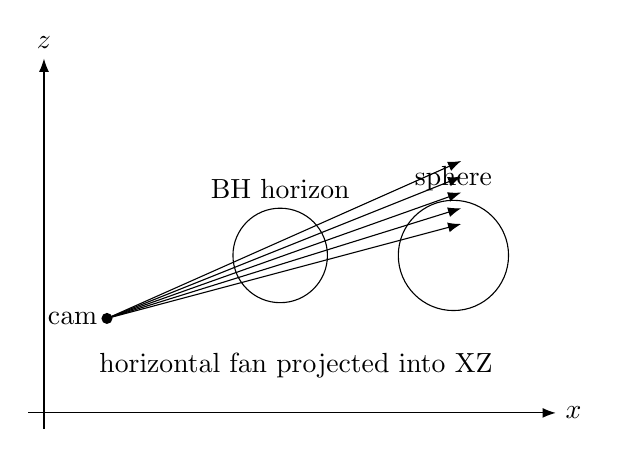
\begin{tikzpicture}[>=Latex, scale=1.0]
  % Axes
  \draw[->] (-0.2,0) -- (6.5,0) node[right] {$x$};
  \draw[->] (0,-0.2) -- (0,4.5) node[above] {$z$};

  % BH circle
  \draw (3,2) circle (0.6);
  \node[above] at (3,2.6) {BH horizon};

  % Sphere circle
  \draw (5.2,2) circle (0.7);
  \node[above] at (5.2,2.7) {sphere};

  % Camera
  \fill (0.8,1.2) circle (2pt);
  \node[left] at (0.8,1.2) {cam};

  % Rays fan
  \foreach \a in {-20,-10,0,10,20} {
    \draw[->] (0.8,1.2) -- ++(4.5, {1.6 + 0.02*\a});
  }

  \node at (3.2,0.6) {horizontal fan projected into XZ};
\end{tikzpicture}
\caption{The debug split view projects ray paths into the XZ plane for top-down inspection.}
\end{figure}


\section{Conceptual Summary}

\begin{itemize}
\item One ray per pixel.
\item All rays originate at a single point.
\item The image plane defines directions, not positions.
\item Ray marching advances all rays in parallel.
\item Camera up vector is a preference, not a constraint.
\end{itemize}




\end{document}

